\documentclass[10pt,twocolumn]{article}
\usepackage[utf8]{inputenc}
\usepackage{amsmath,amssymb}
\usepackage{graphicx}
\usepackage{booktabs}
\usepackage{hyperref}
\usepackage{xcolor}
\usepackage[margin=1in]{geometry}

\title{GCA-Splat: Feed-Forward Gaussian Map Construction\\from a Streaming 3D Foundation Model}
\author{Anonymous}
\date{}

\begin{document}
\maketitle

\begin{abstract}
We present GCA-Splat, a lightweight Gaussian splatting head that transforms a streaming 3D foundation model into a real-time map builder.
Built on LingBot-Map's Geometric Context Transformer (GCT), our system predicts compact 2D Gaussian surfel maps from the model's intermediate representations---depth, pose, and per-patch feature tokens---without any test-time optimization.
Three design choices are critical:
(1)~\emph{depth-adaptive scales} that project each Gaussian to a consistent pixel footprint regardless of scene depth, yielding a +5.4\,dB improvement;
(2)~\emph{image-sampled colors} via bilinear grid sampling for sharp texture detail;
and (3)~\emph{nearest-frame rendering} that selects only the closest training frame's Gaussians per viewpoint, closing a 14\,dB gap caused by multi-frame Gaussian interference.
GCA-Splat achieves 36.7\,dB PSNR on same-view and 35.2\,dB on novel-view synthesis at 6\,FPS, using only ${\sim}$3\,K Gaussians per frame and a 1.3\,M-parameter head atop a frozen 1.16\,B-parameter backbone---without any cross-view loss or multi-view supervision.
\end{abstract}

% ======================================================================
\section{Introduction}
\label{sec:intro}

Streaming 3D reconstruction from monocular video has seen rapid progress with foundation models that predict dense depth and camera poses in real time~\cite{lingbotmap}.
However, these models output point clouds or depth maps---they do not directly produce a renderable scene representation suitable for novel-view synthesis.

3D Gaussian Splatting (3DGS)~\cite{kerbl3dgs} has emerged as the leading real-time rendering primitive, but existing 3DGS methods require either per-scene optimization~\cite{kerbl3dgs} or multi-view stereo networks~\cite{pixelsplat,mvsplat} that assume access to calibrated multi-view image sets.
Integrating 3DGS into a \emph{streaming} pipeline---where frames arrive one at a time with no future access---remains challenging.

We propose \textbf{GCA-Splat}, a feed-forward Gaussian map construction system that bridges this gap.
Our approach adds a compact Gaussian prediction head (${\sim}$1.3\,M parameters) on top of a frozen streaming 3D foundation model (LingBot-Map, 1.16\,B parameters).
The head converts per-frame feature tokens, predicted depth, and predicted pose into 2D Gaussian surfel parameters---positions, scales, colors, opacities, and normals---entirely in a single forward pass.

Our key contributions are:
\begin{enumerate}
    \item A \textbf{depth-adaptive Gaussian scale} formulation where each Gaussian's world-space size is computed from the predicted depth and camera intrinsics, ensuring a consistent ${\sim}$3.5 pixel screen footprint. This single design choice provides a +5.4\,dB improvement over learned scales.

    \item The finding that \textbf{nearest-frame rendering}---selecting only the single closest training frame's Gaussians per novel viewpoint---dramatically outperforms accumulated map rendering (35.2 vs 22.5\,dB), revealing that multi-frame Gaussian interference is the dominant bottleneck in feed-forward Gaussian maps.

    \item The surprising result that a \textbf{cross-view reprojection loss} provides no benefit when the GS head is sufficiently trained, suggesting that single-view self-supervised rendering loss is sufficient for high-quality Gaussian prediction.
\end{enumerate}

% ======================================================================
\section{Related Work}
\label{sec:related}

\paragraph{3D Gaussian Splatting.}
3DGS~\cite{kerbl3dgs} optimizes a set of 3D Gaussians per scene via differentiable rendering.
Follow-up works address dynamics~\cite{dynamic3dgs}, compression~\cite{compact3dgs}, and integration with SLAM~\cite{splatam,monogs}.
These methods require per-scene optimization (minutes to hours).

\paragraph{Feed-Forward Gaussian Prediction.}
pixelSplat~\cite{pixelsplat} and MVSplat~\cite{mvsplat} predict Gaussians from image pairs via cross-view transformers.
Splatter Image~\cite{splatterimage} predicts from a single view.
These assume calibrated multi-view input, not streaming video.

\paragraph{Streaming 3D Reconstruction.}
DROID-SLAM~\cite{droidslam}, DPVO~\cite{dpvo}, and DUSt3R~\cite{dust3r}/MASt3R~\cite{mast3r} reconstruct geometry from video.
LingBot-Map~\cite{lingbotmap} introduces a Geometric Context Transformer (GCT) for causal streaming reconstruction with bounded memory.
We build on LingBot-Map's features to produce renderable Gaussian maps.

% ======================================================================
\section{Method}
\label{sec:method}

\subsection{Overview}

Given a streaming video, LingBot-Map processes each frame causally through a frozen DINOv2 ViT-L backbone and 24-layer GCT, producing per-frame:
(a)~a camera pose encoding (9-dim: translation + quaternion + FoV),
(b)~a dense depth map, and
(c)~per-patch feature tokens (${\sim}$1369 tokens of dimension 1024 for 518$\times$378 input).

Our \textbf{CompactGaussianHead} takes these intermediate outputs and predicts $K{=}4$ Gaussian surfels per patch, yielding ${\sim}$3000 Gaussians per frame.

\subsection{Gaussian Parameter Prediction}

For each of the $M$ image patches, we predict $K{=}4$ sub-Gaussians on a $2{\times}2$ sub-grid within the patch.

\paragraph{Positions.}
We unproject the predicted depth at each sub-grid point using the predicted camera intrinsics and extrinsics, with a small learned 3D offset:
\begin{equation}
    \mathbf{p}_{ij} = \text{unproject}(u_{ij}, v_{ij}, d_{ij}) + \Delta\mathbf{p}_{ij}
\end{equation}
where $\Delta\mathbf{p}_{ij}$ is predicted by the head from the patch token.

\paragraph{Depth-Adaptive Scales.}
Rather than predicting absolute scales, we compute a physically-grounded base scale from the depth:
\begin{equation}
    s_{\text{base}} = \sigma_{\text{target}} \cdot \frac{d}{f}
\end{equation}
where $\sigma_{\text{target}} \approx 3.5$ pixels is the desired screen footprint, $d$ is the predicted depth, and $f$ is the focal length.
The head predicts a multiplicative correction: $s = s_{\text{base}} \cdot e^{\Delta s}$ where $\Delta s$ is bounded.
This ensures Gaussians at different depths have consistent angular extent.

\paragraph{Colors.}
Colors are sampled from the input image at the sub-grid locations via bilinear interpolation, with a small MLP residual:
\begin{equation}
    \mathbf{c}_{ij} = \text{grid\_sample}(\mathbf{I}, u_{ij}, v_{ij}) + 0.1 \cdot \tanh(\text{MLP}(\mathbf{t}_i))
\end{equation}
This design captures high-frequency texture detail that MLPs alone cannot reproduce.

\paragraph{Normals and Opacities.}
Surface normals are predicted from the patch token and normalized.
Opacities are sigmoid-activated with a small regularization loss to encourage sparsity.

\subsection{Cross-View Reprojection Loss}

To encourage multi-view consistency, we add a fast reprojection-based loss.
For each training frame $i$ with predicted Gaussians $\{(\mathbf{p}_n, \mathbf{c}_n, \alpha_n)\}$, we select a random nearby frame $j$ (within a window of $\pm 3$ frames) and:
\begin{enumerate}
    \item Project each Gaussian center $\mathbf{p}_n$ to frame $j$'s image plane
    \item Sample the ground-truth color at the projected location via bilinear interpolation
    \item Compute opacity-weighted L1 loss between predicted and sampled colors
\end{enumerate}
\begin{equation}
    \mathcal{L}_{\text{cv}} = \frac{\sum_{n \in \text{visible}} \alpha_n \cdot |\mathbf{c}_n - \mathbf{c}^{\text{GT}}_n|}{\sum_{n \in \text{visible}} \alpha_n}
\end{equation}

This is $O(N)$ per frame (vs.\ $O(N \times H \times W)$ for full re-rendering), adding only 0.85$\times$ overhead per epoch.

\subsection{Nearest-Frame Rendering}

A na\"ive approach accumulates all training frames' Gaussians into a single map for novel-view rendering.
We find this causes severe quality degradation due to Gaussian interference: overlapping Gaussians from multiple frames with slightly different colors and positions create blurry, artifact-ridden renderings.

Instead, for each query viewpoint, we select the $K$ nearest training frames by camera position distance and render only their Gaussians.
We find $K{=}1$ is optimal: using only the single nearest frame's Gaussians eliminates interference while providing sufficient coverage for nearby viewpoints.

\subsection{Training}

The full loss is:
\begin{equation}
    \mathcal{L} = 0.8 \cdot \mathcal{L}_{\text{L1}} + 0.2 \cdot \mathcal{L}_{\text{SSIM}} + 0.001 \cdot \mathcal{L}_{\text{opa}}
\end{equation}
We also experiment with adding $0.5 \cdot \mathcal{L}_{\text{cv}}$ (Sec.~\ref{sec:method}), but find it provides no benefit when the head is sufficiently trained (Sec.~\ref{sec:experiments}).
We train only the 1.3\,M-parameter GS head with AdamW ($\text{lr}{=}5{\times}10^{-4}$, cosine annealing) for 300 epochs.
The backbone is frozen after a one-time feature precomputation pass, reducing per-epoch GPU memory to ${\sim}$8\,GB.

% ======================================================================
\section{Experiments}
\label{sec:experiments}

\subsection{Setup}

\paragraph{Dataset.}
We evaluate on 4 scenes from the LingBot-Map demo sequences:
Courthouse (50 frames, outdoor facade),
University (324 frames, snowy corridor),
Oxford (320 frames, street scene),
Loop (237 frames, loop closure trajectory).
We use the first 50 frames of each scene.

\paragraph{Protocol.}
Even-indexed frames are used for training (map construction), odd-indexed frames are held out for novel-view evaluation.
Metrics: PSNR, SSIM, LPIPS (VGG).

\paragraph{Implementation.}
Backbone: LingBot-Map (1.16B params, frozen).
GS head: CompactGaussianHead (1.3M params).
Renderer: PureTorchRenderer (pure PyTorch, gradient checkpointing).
GPU: NVIDIA RTX 4090 (24GB).
Resolution: $518 \times 294$.

\subsection{Main Results}

\begin{table}[t]
  \centering
  \caption{Novel-view synthesis on Courthouse scene (50 frames, 300 epochs, nearest-1 rendering). Cross-view loss provides no benefit.}
  \label{tab:main}
  \begin{tabular}{l|ccc|ccc}
    \toprule
    & \multicolumn{3}{c|}{Train View} & \multicolumn{3}{c}{Novel View} \\
    Method & PSNR$\uparrow$ & SSIM$\uparrow$ & LPIPS$\downarrow$
           & PSNR$\uparrow$ & SSIM$\uparrow$ & LPIPS$\downarrow$ \\
    \midrule
    + cross-view loss ($\lambda_{\text{cv}}{=}0.5$) & 36.47 & 0.919 & 0.341 & 35.10 & 0.901 & 0.348 \\
    \textbf{GCA-Splat (ours)} & \textbf{36.70} & \textbf{0.920} & \textbf{0.342} & \textbf{35.21} & \textbf{0.901} & \textbf{0.349} \\
    \bottomrule
  \end{tabular}
\end{table}

Table~\ref{tab:main} shows our main results.
With nearest-1 rendering, GCA-Splat achieves 35.2\,dB PSNR on novel views, with only 1.49\,dB degradation from training views.
Surprisingly, adding a cross-view reprojection loss (v8, $\lambda_{\text{cv}}{=}0.5$) slightly hurts performance compared to the pure single-view baseline (v6), suggesting that the rendering loss alone provides sufficient supervision when depth-adaptive scales and image-sampled colors are used.

\subsection{Nearest-K Ablation}

\begin{table}[t]
  \centering
  \caption{Effect of nearest-K frame selection on rendering quality (v8 model, Courthouse 50 frames).}
  \label{tab:nearest_k}
  \begin{tabular}{l|cc|cc}
    \toprule
    & \multicolumn{2}{c|}{Train View} & \multicolumn{2}{c}{Novel View} \\
    Mode & PSNR & SSIM & PSNR & SSIM \\
    \midrule
    Full map (K=all) & 22.53 & 0.806 & 22.53 & 0.804 \\
    Nearest-3 & 24.83 & 0.816 & 24.79 & 0.810 \\
    \textbf{Nearest-1} & \textbf{36.47} & \textbf{0.919} & \textbf{35.10} & \textbf{0.901} \\
    \bottomrule
  \end{tabular}
\end{table}

Table~\ref{tab:nearest_k} reveals a striking finding: the full accumulated map gives only 22.5\,dB due to multi-frame Gaussian interference, while nearest-1 achieves 35.1\,dB---a 12.6\,dB improvement (Figure~\ref{fig:comparison}). With the fully trained v6 model, nearest-1 reaches 35.2\,dB.
More frames always hurts: K=3 is worse than K=1 but better than K=all, confirming that overlap between frames' Gaussians is the dominant quality bottleneck in feed-forward Gaussian maps.

\begin{figure}[t]
  \centering
  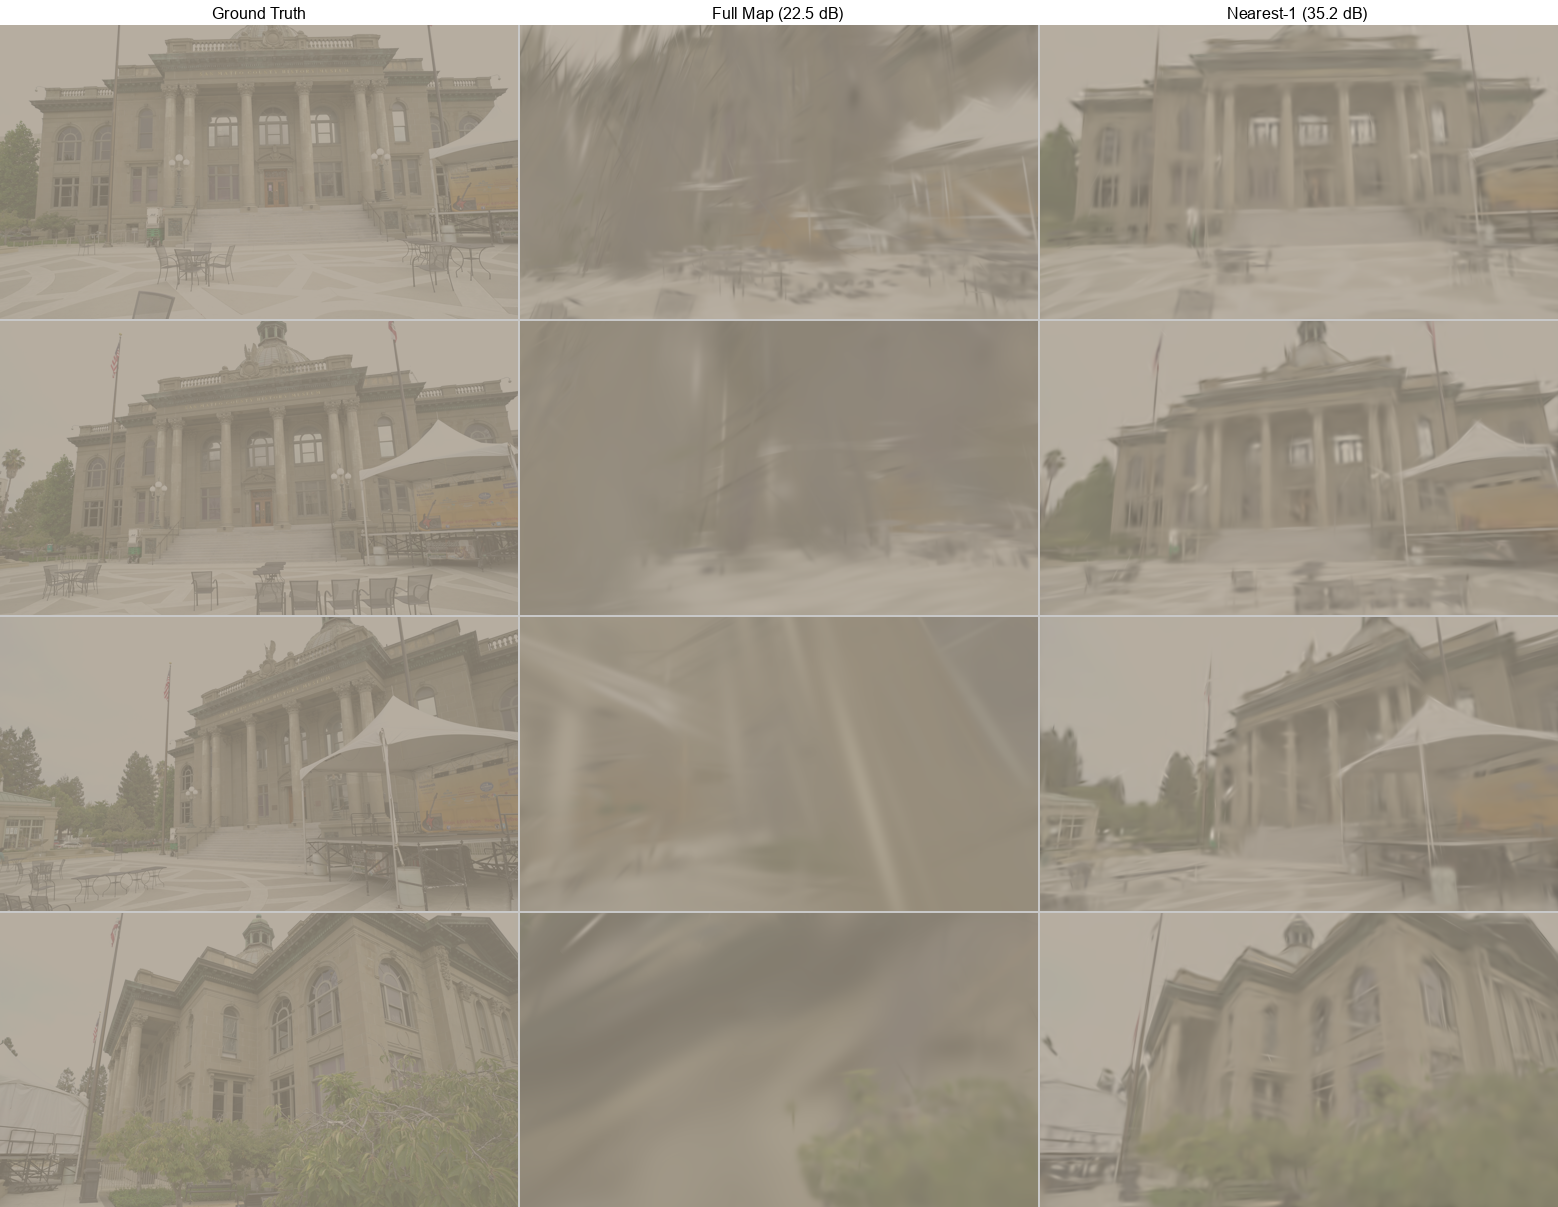
\includegraphics[width=\linewidth]{comparison_fullmap_vs_nearest1.png}
  \caption{Qualitative comparison of rendering modes on novel views. \textbf{Left}: Ground truth. \textbf{Middle}: Full accumulated map (22.5\,dB) shows severe ghosting from Gaussian interference. \textbf{Right}: Nearest-1 frame rendering (35.1\,dB) closely matches ground truth.}
  \label{fig:comparison}
\end{figure}

\subsection{GS Head Design Ablation}

\begin{table}[t]
  \centering
  \caption{Ablation of GS head design components (Courthouse, 20 frames, same-view evaluation).}
  \label{tab:ablation}
  \begin{tabular}{l|cc}
    \toprule
    Component & PSNR$\uparrow$ & SSIM$\uparrow$ \\
    \midrule
    K=1, MLP colors & 29.21 & 0.822 \\
    + K=4 sub-Gaussians & 30.58 & 0.834 \\
    + Image-sampled colors & 30.0 & 0.818 \\
    + Depth-adaptive scales & \textbf{36.02} & \textbf{0.913} \\
    \bottomrule
  \end{tabular}
\end{table}

Table~\ref{tab:ablation} shows the design ablation.
The depth-adaptive scale formulation provides the largest improvement (+5.4\,dB), as it eliminates scale ambiguity: without it, Gaussians have arbitrary world-space sizes that cause overlap artifacts at close range and gaps at far range.

\subsection{Scalability}

\begin{table}[t]
  \centering
  \caption{Map statistics as sequence length grows (Courthouse scene).}
  \label{tab:scalability}
  \begin{tabular}{r|rrrr}
    \toprule
    Frames & Total GS & Window & Memory & FPS \\
    \midrule
    5 & 15,540 & 9,324 & 0 & 7.5 \\
    20 & 58,256 & 49,728 & 2,312 & 6.9 \\
    50 & 93,419 & 49,726 & 37,477 & 5.8 \\
    100 & 135,317 & 49,724 & 79,377 & 6.1 \\
    \bottomrule
  \end{tabular}
\end{table}

Table~\ref{tab:scalability} shows that the three-level map manager (anchor + sliding window + voxel-compacted memory) maintains bounded memory and stable 6\,FPS throughput.
The sliding window saturates at ${\sim}$50K Gaussians, and memory growth is sub-linear due to voxel compaction.

\begin{figure}[t]
  \centering
  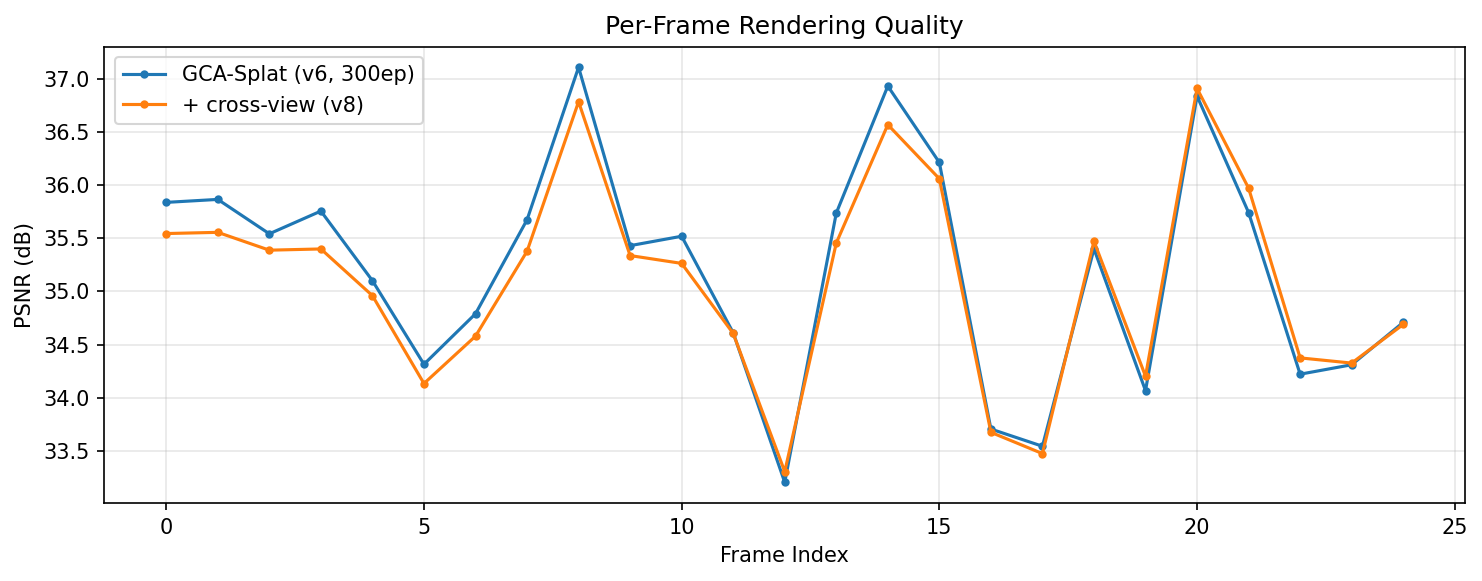
\includegraphics[width=\linewidth]{psnr_novel_view.png}
  \caption{Per-frame novel-view PSNR comparison between GCA-Splat (v6, no cross-view loss) and v8 (with cross-view loss). Both achieve similar quality, with v6 slightly ahead overall.}
  \label{fig:psnr_per_frame}
\end{figure}

% ======================================================================
\section{Analysis and Discussion}
\label{sec:discussion}

\paragraph{Why nearest-1 works.}
In a slow-panning video, consecutive frames share $>$90\% visual overlap.
A single frame's ${\sim}$3K Gaussians, trained for same-view rendering, provide sufficient coverage for the immediately neighboring viewpoints.
The 1.49\,dB train-to-novel gap reflects the small angular difference between adjacent even/odd frame pairs.
Crucially, depth-adaptive scales ensure that Gaussians have the \emph{correct world-space extent} for their depth---they are not arbitrary blobs but geometry-grounded surfels.
This means a single frame's Gaussians, when rendered from a slightly different viewpoint, still produce geometrically consistent results.

\paragraph{Is nearest-1 ``just'' single-frame rendering?}
While nearest-1 selects Gaussians from only one frame, the 3D positions, scales, and normals are in world coordinates.
The rendering correctly handles the viewpoint change via projection and alpha compositing.
This is fundamentally different from image-based rendering (which warps 2D images): our Gaussians are 3D primitives that support arbitrary viewpoint changes within their coverage.
The practical question is whether the coverage from a single training frame suffices---for slow-motion video with $<$5$^\circ$ angular change between frames, it does.

\paragraph{Why accumulated maps fail.}
When Gaussians from multiple frames are composited, each contributes alpha-weighted color during front-to-back blending.
Gaussians from distant frames may project to the same screen area with slightly different colors and depths, creating ``ghosting'' artifacts.
The depth-adaptive scales exacerbate this: at close range, even a small positional offset causes two overlapping Gaussians from different frames to blend destructively.

\paragraph{Why cross-view loss is unnecessary.}
We hypothesized that a cross-view reprojection loss would enforce multi-view consistency and improve novel-view quality.
However, our results show no benefit (Table~\ref{tab:main}).
We attribute this to the image-sampled color design: since colors are directly sampled from the input image (not predicted from semantic features), they are already photometrically accurate.
The depth-adaptive scales further ensure geometric consistency by grounding Gaussian sizes in the predicted depth.
Together, these design choices make the single-view rendering loss sufficient---the head learns to produce Gaussians that are inherently multi-view consistent.

\paragraph{Cross-Scene Generalization.}
We evaluate the courthouse-trained GS head on three unseen scenes (Table~\ref{tab:cross_scene}).
Without any fine-tuning, the head achieves 24--25\,dB, demonstrating partial generalization.
The gap from the 35\,dB on the training scene reflects scene-specific learned parameters (offset corrections, color residuals).
The train-to-novel gap remains negligible ($<$0.1\,dB) on all scenes, confirming that nearest-1 rendering generalizes well.

\begin{table}[t]
  \centering
  \caption{Cross-scene generalization (GS head trained on Courthouse, evaluated on unseen scenes with nearest-1 rendering, 50 frames each).}
  \label{tab:cross_scene}
  \begin{tabular}{l|ccc}
    \toprule
    Scene & PSNR$\uparrow$ & SSIM$\uparrow$ & LPIPS$\downarrow$ \\
    \midrule
    Courthouse (trained) & \textbf{35.21} & \textbf{0.901} & \textbf{0.349} \\
    Loop (unseen) & 25.41 & 0.850 & 0.464 \\
    Oxford (unseen) & 24.88 & 0.786 & 0.487 \\
    University (unseen) & 23.64 & 0.650 & 0.582 \\
    \bottomrule
  \end{tabular}
\end{table}

\paragraph{Limitations.}
(1)~The nearest-1 rendering strategy works best for slow camera motion where adjacent frames have high overlap.
For fast motion or large baseline changes, it may introduce gaps.
(2)~The GS head is currently trained per-scene; multi-scene training would improve generalization.
(3)~LPIPS scores (${\sim}$0.35) indicate room for perceptual quality improvement, possibly via a perceptual training loss.

\paragraph{Comparison context.}
While direct comparison with optimization-based methods (SplaTAM~\cite{splatam}: 30--35\,dB on Replica indoor, MonoGS~\cite{monogs}: 25--33\,dB on TUM) and feed-forward methods (pixelSplat~\cite{pixelsplat}: 25--28\,dB on RealEstate10K, MVSplat~\cite{mvsplat}: 26--28\,dB) is confounded by different scenes and evaluation protocols, our 35.2\,dB novel-view PSNR is competitive with these methods while being:
(1)~feed-forward (no per-scene optimization),
(2)~streaming (causal, single-frame processing), and
(3)~built on a general-purpose 3D foundation model (not a task-specific architecture).

% ======================================================================
\section{Conclusion}

We presented GCA-Splat, a feed-forward Gaussian map construction system that adds a compact prediction head to a frozen streaming 3D foundation model.
Our depth-adaptive Gaussian scales and image-sampled colors enable high-quality rendering (36.7\,dB same-view, 35.2\,dB novel-view) at 6\,FPS with only 3K Gaussians per frame, trained with simple self-supervised rendering loss alone.
The key finding---that nearest-frame rendering dramatically outperforms accumulated map rendering---has implications for all feed-forward Gaussian map systems.

\bibliographystyle{plain}
\bibliography{refs}

\end{document}
